\documentclass[aspectratio=169%可调屏宽比16:9(169),4:3(43)
,serif,mathserif]{beamer}
\mode<presentation>{
%\usetheme{default}
%\usetheme{AnnArbor}
%\usetheme{Antibes}
%\usetheme{Bergen}
%\usetheme{Berkeley}
%\usetheme{Berlin}
%\usetheme{Boadilla}
%\usetheme{CambridgeUS}
%\usetheme{Copenhagen}
%\usetheme{Darmstadt}
%\usetheme{Dresden}
%\usetheme{Frankfurt}
%\usetheme{Goettingen}
%\usetheme{Hannover}
%\usetheme{Ilmenau}
%\usetheme{JuanLesPins}
%\usetheme{Luebeck}
\usetheme{Madrid}
%\usetheme{Malmoe}
%\usetheme{Marburg}
%\usetheme{Montpellier}
%\usetheme{PaloAlto}
%\usetheme{Pittsburgh}
%\usetheme{Rochester}
%\usetheme{Singapore}
%\usetheme{Szeged}
%\usetheme{Warsaw}
% As well as themes, the Beamer class has a number of color themes
% for any slide theme. Uncomment each of these in turn to see how it
% changes the colors of your current slide theme.
%\usecolortheme{albatross}
%\usecolortheme{beaver}
%\usecolortheme{beetle}
%\usecolortheme{crane}
%\usecolortheme{dolphin}
%\usecolortheme{dove}
%\usecolortheme{fly}
%\usecolortheme{lily}
%\usecolortheme{orchid}
%\usecolortheme{rose}
%\usecolortheme{seagull}
%\usecolortheme{seahorse}
%\usecolortheme{whale}
%\usecolortheme{wolverine}
%\setbeamertemplate{footline} % To remove the footer line in all slides uncomment this line
%\setbeamertemplate{footline}[page number] % To replace the footer line in all slides with a simple slide count uncomment this line
%\setbeamertemplate{navigation symbols}{} % To remove the navigation symbols from the bottom of all slides uncomment this line
}
\usepackage{adjustbox}
\usepackage{indentfirst} 
\usepackage{amsmath, amsfonts, epsfig, xspace}
\usepackage{algorithm,algorithmic}
\usepackage{beamerthemesplit}
\usepackage{booktabs}
\usepackage{bm}
\usepackage{braket}
\usepackage{calligra}
\usepackage[T1]{fontenc}
\usepackage{fontspec}
\usepackage{ctex}
\usepackage{latexsym}
\usepackage{multicol}
\usepackage{multimedia}
\usepackage{calligra} \DeclareMathAlphabet{\mathcalligra}{T1}{calligra}{m}{n} \DeclareFontShape{T1}{calligra}{m}{n}{<->s*[2.2]callig15}{}
\usepackage{pstricks,pst-node}
\usepackage{ragged2e}
\usepackage{setspace}
\usepackage[normal,tight,center]{subfigure}
\setlength{\subfigcapskip}{-.5em}
\setlength{\parindent}{2em}
\begin{document}
\title[Synthesizing Context-free Grammars from Recurrent Neural Networks]{Synthesizing Context-free Grammars from Recurrent Neural Networks} % The short title appears at the bottom of every slide, the full title is only on the title page
\author[Chi~Zhiming]{迟智名} % Your name
\institute[LZU] % Your institution as it will appear on the bottom of every slide, may be shorthand to save space
{	
	%Lanzhou University \\ % Your institution for the title page
	%\medskip
	%\textit{chizhm16@lzu.edu.cn} % Your email address
}
	\CTEXoptions[today=old]
	\date{\today} % Date, can be changed to a custom date
\begin{frame}[plain]\vspace{1.5em}
\titlepage\vspace{-0.5cm}
%\centerline{\includegraphics[height=0.30\textheight]{logo.png}}
%\hfill 指导教师:焦桂梅
\end{frame}
\begin{frame}{目录}
\tableofcontents
\end{frame}
\AtBeginSection[]
{
\begin{frame}{\tiny}
\frametitle{目录}
\tableofcontents[currentsection]
\end{frame}
}
%----------------------------------------------------------------------------------------
%	PRESENTATION SLIDES
%----------------------------------------------------------------------------------------

%------------------------------------------------
\section{Introduction} % Sections can be created in order to organize your presentation into discrete blocks, all sections and subsections are automatically printed in the table of contents as an overview of the talk
%------------------------------------------------
\subsection{Extract CFGs from RNN}
\begin{frame}
	Extract CFGs from RNN
\begin{itemize}		
	\item extracting Automata(DFA sequences) from RNN using $L^*$ algorithm
	\item DFAS $\to$ PRSs(pattern rule sets) $\to$ CFGs  
\end{itemize}

\end{frame}

\subsection{Common knowledge}
\begin{frame}
	\begin{itemize}
		\item DFA: $<\Sigma,q_0,Q,F,\delta>$; $\hat{\delta}\left(q_{1}, wa\right) = \delta(\hat{\delta}\left(q_{1}, w\right))$
		\item Complete DFA: $\forall (q,a) \in Q \times \Sigma, \delta(q,a)$ is defined
		\item Sink reject states: $Q_R$
		\item $L(A, q_{1}, q_{2}) \triangleq\{w \in \Sigma^{*} \mid \hat{\delta}(q_{1}, w)=q_{2}\}$
		\item defined tokens:$def~(A,q) \triangleq \{\sigma \in \Sigma \mid \delta(q, \sigma) \notin Q_{R}\}$
		\item Set Representation of $\delta$:$S_{\delta}=\left\{\left(q, \sigma, q^{\prime}\right) \mid \delta(q, \sigma)=q' \right\}$
		\item Replacing a State: $\delta_{\left[q \leftarrow q_{n}\right]}: Q^{\prime} \times \Sigma \rightarrow Q^{\prime}$
	\end{itemize}
		
\end{frame}

\begin{frame}
	Dyck language of order N:$D ::= \epsilon~|~L_i D R_i~|~DD, 1\leq i \leq N$
	\begin{itemize}
		\item D: Start symbol		
		\item $L_i,R_i$ : matching left and right delimiters
		\item distance \& embedding depth 
	\end{itemize}

	Regular Expression Dyck language:$L_i,R_i$ derive some regular expression
	\begin{itemize}
		\item Regular Expression :$\{a|b\}·c$
		\item The Chomsky–Schützenberger representation theorem shows that any context-free language can be expressed as
		a homomorphic image of a Dyck language intersected with a regular language
	\end{itemize}	
\end{frame}

\subsection{Pattern Rule Sets}
\begin{frame}
	\frametitle{Pattern}
	\begin{definition}[Patterns]
		A pattern~p=$\left\langle\Sigma, q_{0}, Q, q_{X}, \delta\right\rangle$  
		is a DFA  $A^{p}= \left\langle\Sigma, q_{0}, Q,\left\{q_{X}\right\}, \delta\right\rangle$  
		satisfying: $L\left(A^{p}\right) \neq \emptyset$ , and either~$q_{0}=q_{X} $, or 
		$\operatorname{def}\left(q_{X}\right)=\emptyset$ and $L\left(A, q_{0}, q_{0}\right)=\{\varepsilon\} $.  If $q_{0}=q_{X}$ then $ p$ is called circular, otherwise, it is non-circular.
	\end{definition}
	\begin{itemize}
		\item  $L_p  = L(p)$
		\item $p^i =\left\langle\Sigma, q_{0}^i, Q^i, q_{X}^i, \delta^i\right\rangle$  
	\end{itemize}
\end{frame}

\begin{frame}
	\frametitle{Composition}
	\begin{definition}[Serial Composition]
		Let $p^{1}, p^{2}$ be two non-circular patterns. 
		Their serial composite is the pattern $p^{1} \circ p^{2}=\left\langle\Sigma, 
		q_{0}^{1}, Q, q_{X}^{2}, \delta\right\rangle$ 
		in which  $Q = Q^{1} \cup Q^{2} \backslash\left\{q_{X}^{1}\right\}$ and
		$\delta=\delta_{\left[q_{X}^{1}\leftarrow q_{0}^{2}\right]}^{1} \cup \delta^{2}$ . 
		We call~$q_{0}^{2}$~the \textbf{join state} of this operation.
	\end{definition}

\end{frame}

\begin{frame}
	\frametitle{Composition}
	\begin{definition}[Circular Composition]
	Let  $p^{1}, p^{2}$ be two non-circular patterns. 
	Their circular composite is the circular pattern $p_{1} \circ_{c} p_{2}=\langle\Sigma, q_{0}^{1}, Q, q_{0}^{1}, \delta\rangle$  
	in which  $Q=Q^{1} \cup Q^{2} \backslash\left\{q_{X}^{1}, q_{X}^{2}\right\}$ 
	and $\delta=\delta_{\left[q_{X}^{1} \leftarrow q_{0}^{2}\right]}^{1} \cup \delta_{[q_{X}^{2} \leftarrow q_{0}^{1}]}^{2}$.
	We call  $q_{0}^{2}$  the join state of this operation.
	\end{definition}

	\begin{itemize}
		\item $L_p = L_{p_1} \cdot L_{p_2}$
		\item $L_p = \{L_{p_1} \cdot L_{p_2}\}^{*}$
	\end{itemize}
\end{frame}

\begin{frame}
	\frametitle{Composition}
	\begin{figure}
		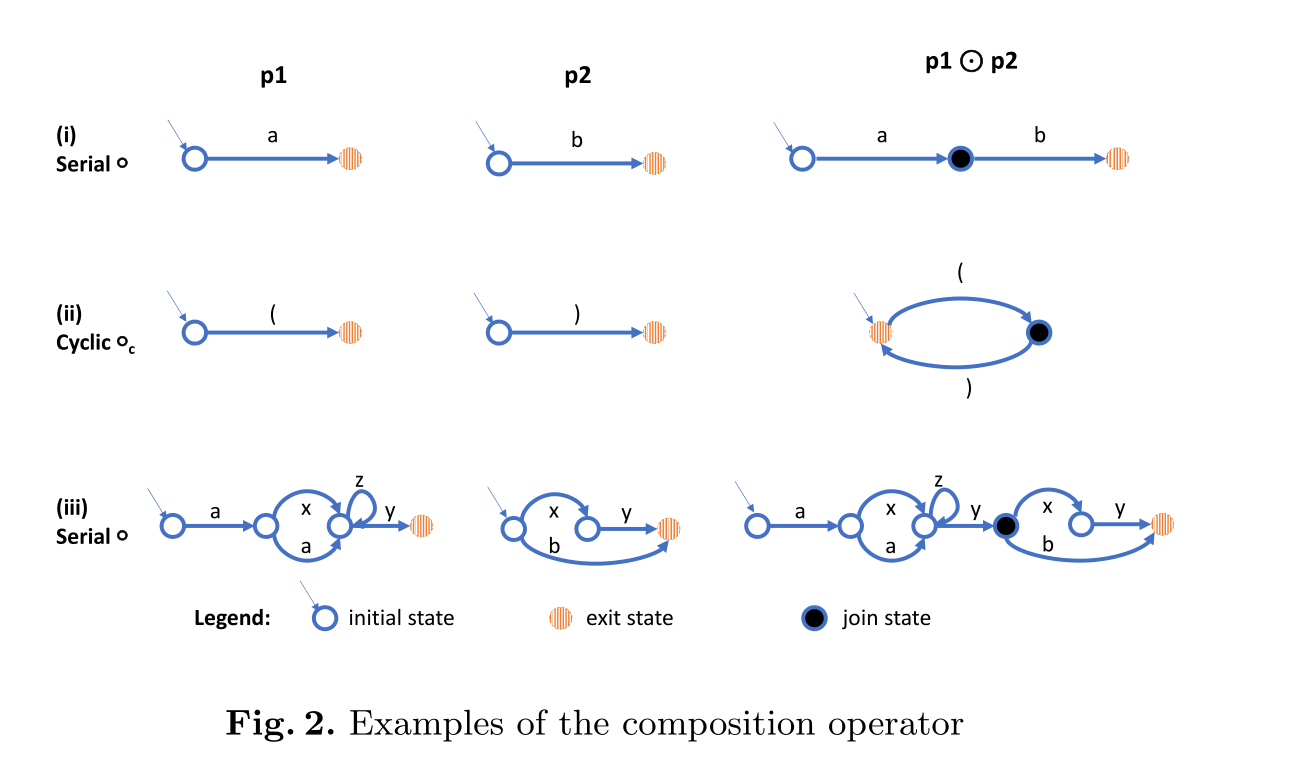
\includegraphics[width=0.8\linewidth]{1.png}
	\end{figure}
\end{frame}
	
\begin{frame}
	\frametitle{Pattern Instances}
	\begin{definition}[Pattern Pair]
		A pattern pair is a pair $\langle P, P_{c}\rangle$ of pattern sets, 
		such that $P_{c} \subset P$  and for every $p \in P_{c}$ 
		there exists exactly one pair $p_{1}, p_{2} \in P$ satisfying  
		$p=p_{1} \odot p_{2}$  for some  $\odot \in \{\circ, \circ_{c} \}$ . 
		We refer to the patterns $p \in P_{c}$ as the \textbf{composite patterns} of  
		$\left\langle P, P_{c}\right\rangle$ , and to the rest as its \textbf{base patterns}.
	\end{definition}

	\begin{definition}[Pattern Instances]
		Let $A=\left\langle\Sigma, q_{0}^{A}, Q^{A}, F, \delta^{A}\right\rangle$  be a DFA,  
		$p=\left\langle\Sigma, q_{0}, Q, q_{X}, \delta\right\rangle$  be a pattern, and
		$\hat{p}=\left\langle\Sigma, q_{0}^{\prime}, Q^{\prime}, q_{X}^{\prime}, \delta^{\prime}\right\rangle$ 
		be a pattern \textbf{inside} $A$ , i.e., $Q^{\prime} \subseteq Q^{A}$ 
		and $\delta^{\prime} \subseteq \delta^{A}$ .  We say that 
		$\hat{p}$  is an instance of  $p$  in  $A$  if  $\hat{p}$  is isomorphic to  $p$ . 
	\end{definition}
\end{frame}

\begin{frame}
	\frametitle{join}
	\begin{definition}[join]
		For each composite pattern $p \in P_c$, DFA $A$, and initial state $q$ of an
instance $\hat{p}$ of $p$ in $A$, $join(p, q, A)$ \textbf{returns the join state of $\hat{p}$} 
with respect to its composition in $<P, P_c>$.
	\end{definition}

	\begin{itemize}
		\item A pattern instance $\hat{p}$  in a DFA $A$ is uniquely determined by its structure and
		initial state: $(p,q)$
	\end{itemize}
\end{frame}

\begin{frame}
	\frametitle{PRS}
	For infinite DFA sequence $S = \{A_1,A_2,\cdots\}, i \in \mathbb{N},L(A_i) \subset L(A_{i+1})$,
	$L(S) = \bigcup\limits_{i = 1}^{\infty} L(A_i)$

	\begin{itemize}
		\item May be used to express CFLs,such as $L=\{{a}^{n}{b}^{n} \mid n \in \mathbb{N}\}$
		\item infinite $\to$ finite : finite prefix, noisy; reconstruct the language by guessing how the sequence may continue
	\end{itemize}

	Pattern rule sets (PRSs): Create sequences of DFAs with a single accepting state.

	\begin{itemize}
		\item Connect a new pattern instance to the current DFA to a join state of composite pattern$A_i$
	\end{itemize}
\end{frame}

\begin{frame}
	\frametitle{PRS}
	\begin{definition}[enabled instances]
		An enabled DFA over a pattern pair  $\left\langle P, P_{c}\right\rangle$  
		is a tuple  $\langle A, \mathcal{I}\rangle$  such that  
		$A=\left\langle\Sigma, q_{0}, Q, F, \delta\right\rangle$  is a DFA and  
		$\mathcal{I} \subseteq P_{c} \times Q$  
		marks \textbf{enabled instances} of composite patterns in A.
	\end{definition}
	 
	Given enabled DFA $<A, I>, (p,q) \in I$:
	\begin{itemize}
		\item  There is an instance of pattern $p$ in $A$ starting at state $q$
		\item  We may connect new pattern instances to its join state join(p, q, A).
	\end{itemize}
\end{frame}

\begin{frame}
	\frametitle{PRS}
	\begin{definition}[Pattern rule sets]
		A PRS  $\mathbf{P}$  is a tuple $\left\langle\Sigma, P, P_{c}, R\right\rangle$  
		where  $\left\langle P, P_{c}\right\rangle$  is a pattern pair over the alphabet
		$\Sigma$  and $R$  is a set of rules. Each rule has one of the following forms, 
		for some  $p, p^{1}, p^{2}, p^{3}, p^{I} \in P$ , with $ p^{1}$  and  $p^{2}$  
		non-circular:
		(1)$\perp \rightarrow p^{I}$ 
		(2)$ p \rightarrow_{c}\left(p^{1} \odot p^{2}\right) \propto p^{3} , where~p=p^{1} \odot p^{2}~for~\odot \in\left\{o, o_{c}\right\} , and~p^{3}~is~circular$
		(3)$ p \rightarrow_{s}\left(p^{1} \circ p^{2}\right) \propto p^{3} , where~p=p^{1} \circ p^{2}~and~p^{3}~is~non-circular$
	\end{definition}
\end{frame}

\begin{frame}
	\frametitle{PRS}
	\begin{definition}[Initial Composition]
		$\mathcal{D}_{1}=\left\langle A_{1}, \mathcal{I}_{1}\right\rangle$ is generated from a rule
		$\perp \rightarrow p^{I}$ as follows: $A_{1}=A^{p^{I}}$, and 
		$\mathcal{I}_{i}=\{\left(p^{I}, q_{0}^{I}\right)\}$ if 
		$p^{I} \in P_{c}$ and otherwise $\mathcal{I}_{1}=\emptyset$.
	\end{definition}

	\begin{definition}[Rules of type (1)]
		A rule $\perp \rightarrow p^{I}$ with circular $p^{I}$ may extend $\left\langle A_{i}, \mathcal{I}_{i}\right\rangle$ at the initial state $q_{0}$ of $A_{i}$.
		iff $\operatorname{def}\left(q_{0}\right)\cap\operatorname{def}\left(q_{0}^{I}\right)=\emptyset$. 
		This creates the DFA $A_{i+1}=\left\langle\Sigma, q_{0}, Q \cup Q^{I} \backslash\{q_{0}^{I}\}, F, \delta \cup \delta_{[q_{0}^{I} \leftarrow q_{0}]}^{I}\right\rangle$.
		If $p^{I}\in P_{c}$ then $\mathcal{I}_{i+1}=\mathcal{I}_{i} \cup\left\{(p^{I}, q_{0})\right\}$
		else $\mathcal{I}_{i+1}=\mathcal{I}_{i}$.
	\end{definition}

\end{frame}

\begin{frame}
	\frametitle{PRS}
	\begin{definition}[Rules of type (2)]
		A rule $p \rightarrow_{c}\left(p^{1} \odot p^{2}\right) \propto p^{3}$ may extend
		$\left\langle A_{i}, \mathcal{I}_{i}\right\rangle $at the join state $q_{j}=\mathrm{join}\left(p, q, A_{i}\right)$
		of any instance $(p, q) \in \mathcal{I}_{i}$, provided 
		$\operatorname{def}\left(q_{j}\right) \cap \operatorname{def}\left(q_{0}^{3}\right)=\emptyset$.
		This creates $\left\langle A_{i+1}, \mathcal{I}_{i+1}\right\rangle$ 
		as follows: $A_{i+1}=\left\langle\Sigma, q_{0}, Q \cup Q^{3} \backslash q_{0}^{3}, F, \delta \cup \delta_{\left[q_{0}^{3} \leftarrow q_{j}\right]}^{3}\right\rangle$, 
		and $\mathcal{I}_{i+1}=\mathcal{I}_{i} \cup \{(p^{k}, q^{k}) \mid p^{k} \in P_{c}, k \in\{1,2,3\}\}$, 
		where $q^{1}=q$ and $q^{2}=q^{3}=q_{j}$
	\end{definition}
\end{frame}

\begin{frame}
	\frametitle{PRS}
	\begin{definition}[Rules of type (3)]
		A rule $p \rightarrow_{s}\left(p^{1} \odot p^{2}\right) \propto p^{3}$ may extend
		$\left\langle A_{i}, \mathcal{I}_{i}\right\rangle $at the join state $q_{j}=\mathrm{join}\left(p, q, A_{i}\right)$
		of any instance $(p, q) \in \mathcal{I}_{i}$, provided 
		$\operatorname{def}(q_{j}) \cap \operatorname{def}\left(q_{0}^{3}\right)=\emptyset$.
		This creates $\left\langle A_{i+1}, \mathcal{I}_{i+1}\right\rangle$ 
		as follows: $A_{i+1}=\left\langle\Sigma, q_{0}, Q \cup Q^{3} \backslash q_{0}^{3}, F, \delta \cup \delta_{\left[q_{0}^{3} \leftarrow q_{j}\right]}^{3} \cup C\right\rangle$
		where $C  = \{(q_{X}^{3}, \sigma, \delta(q_{j}, \sigma)) \mid \sigma \in \operatorname{def}(p^{2}, q_{0}^{2})\}$ is \textbf{connection transitions}, 
		and $\mathcal{I}_{i+1}=\mathcal{I}_{i} \cup \{(p^{k}, q^{k}) \mid p^{k} \in P_{c}, k \in\{1,2,3\}\}$, 
		where $q^{1}=q$ and $q^{2}=q^{3}=q_{j}$
	\end{definition}
\end{frame}

\begin{frame}
	\frametitle{PRS}
	\begin{figure}
		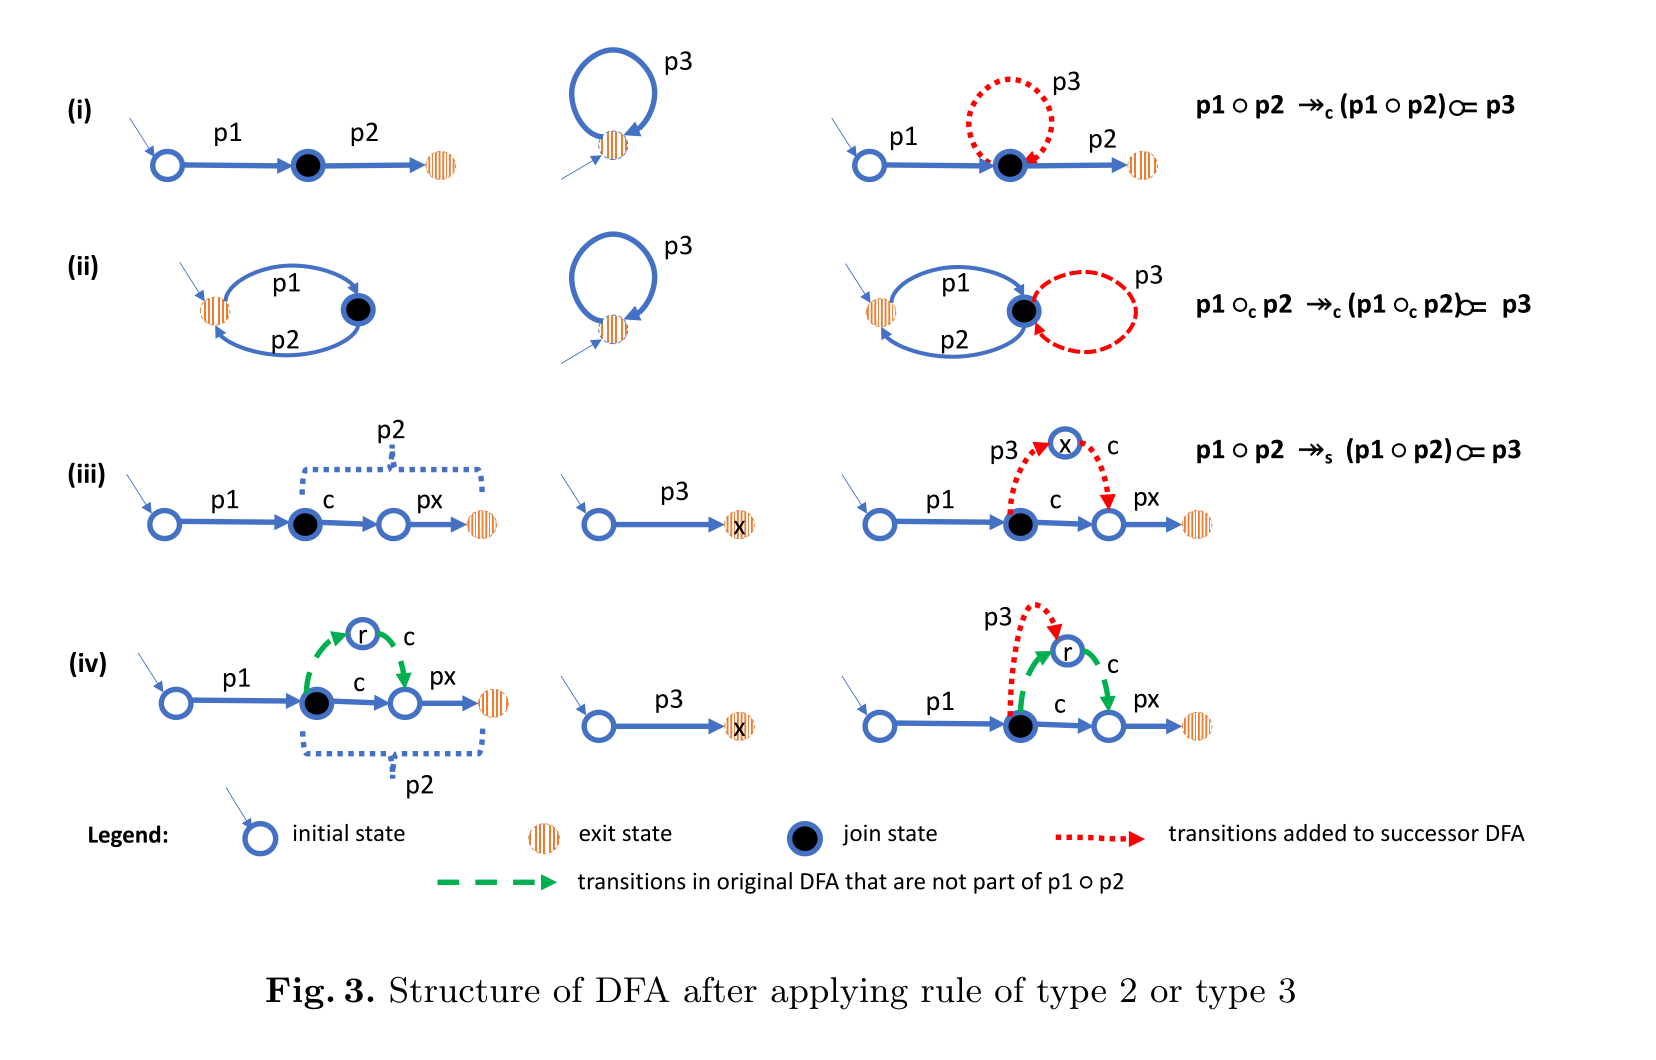
\includegraphics[width=0.8\linewidth]{2.png}
	\end{figure}

	\begin{itemize}
		\item $|F| = 1$
		\item DFAs Generated by a PRS: $A \in G(\mathbf{P})$
		\item Language of a PRS: $L(S) = \bigcup\limits_{A \in G(\mathbf{P})} L(A)$
	\end{itemize}
\end{frame}

\subsection{Example}

\begin{frame}
	\frametitle{Example}
	\begin{figure}
		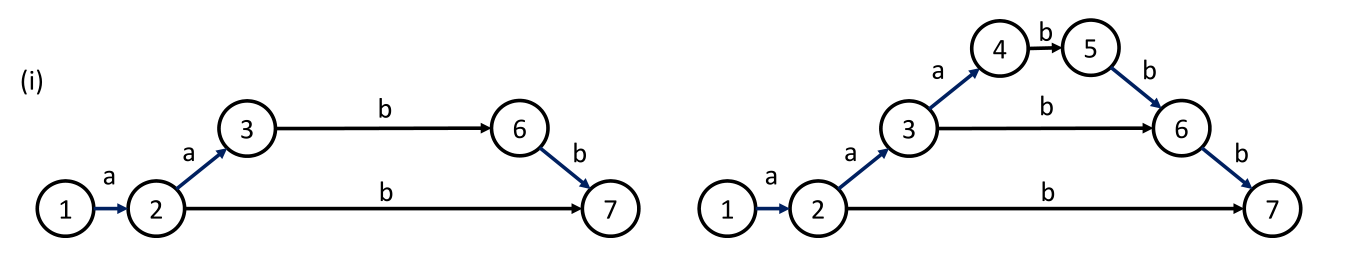
\includegraphics[width=0.8\linewidth]{3.png}
	\end{figure}

	\begin{itemize}
		\item $\perp \rightarrow p^{1} \circ p^{2}$
		\item $p^{1} \circ p^{2} \rightarrow_{s}  (p^{1} \circ p^{2}) \odot (p^{1} \circ p^{2})$
	\end{itemize}	
\end{frame}



%------------------------------------------------


%------------------------------------------------

%------------------------------------------------

\section{PRS Inference Algorithm}
\subsection{Dual problem}
\begin{frame}
\frametitle{Dual problem}
Given DFAs, how to reconstruct PRS $\mathbf{P}$?
\begin{figure}
	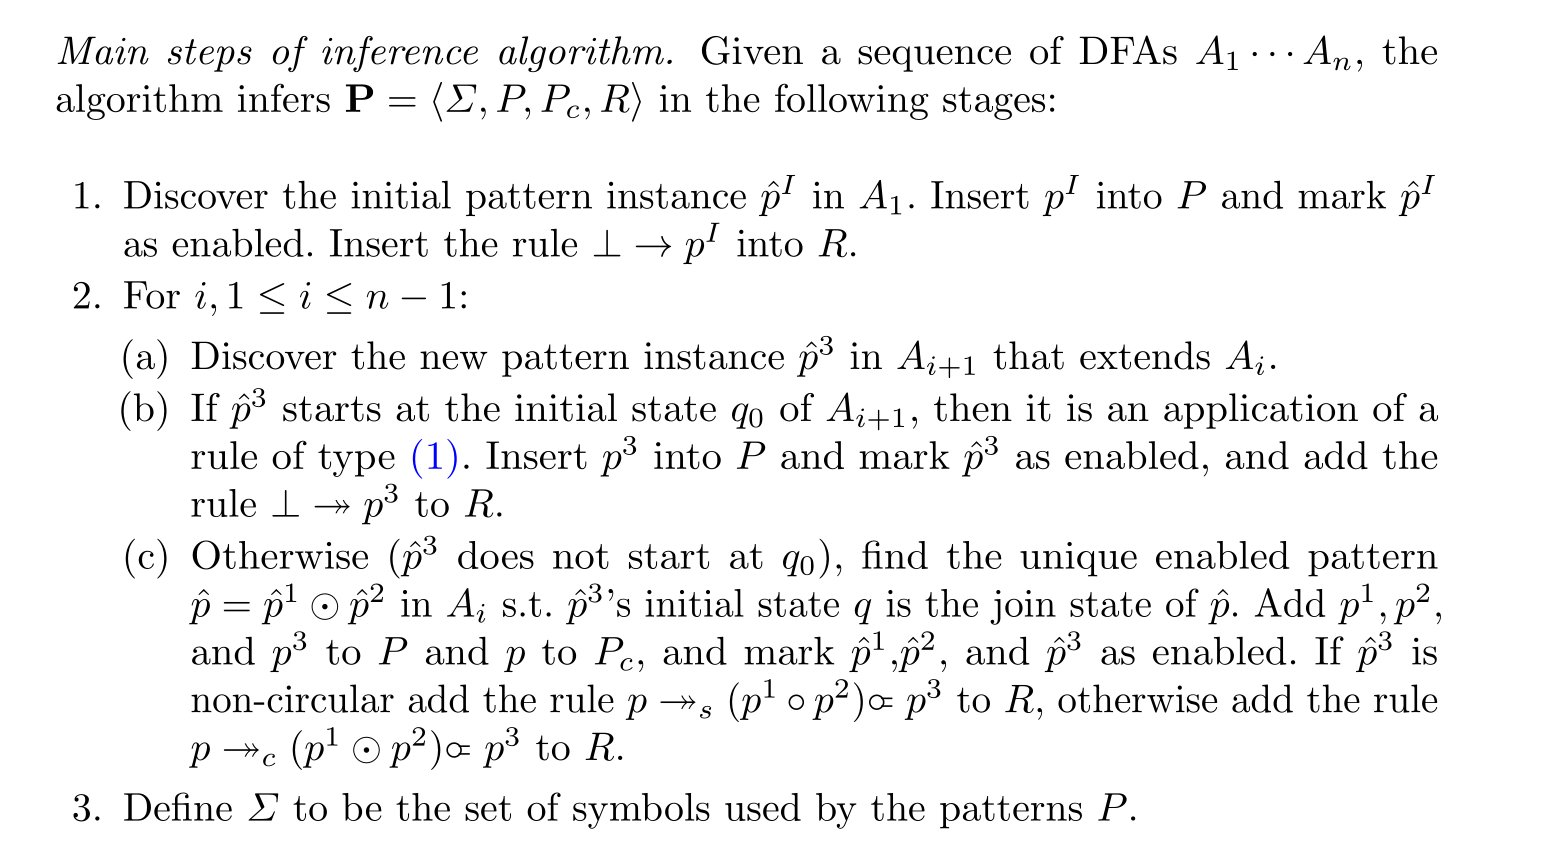
\includegraphics[width=0.6\linewidth]{5.png}
\end{figure}

\end{frame}

\subsection{Questions}
\begin{frame}
	\frametitle{How to Discovering new Patterns}
	Exit State Discovery algorithm
	\begin{figure}
		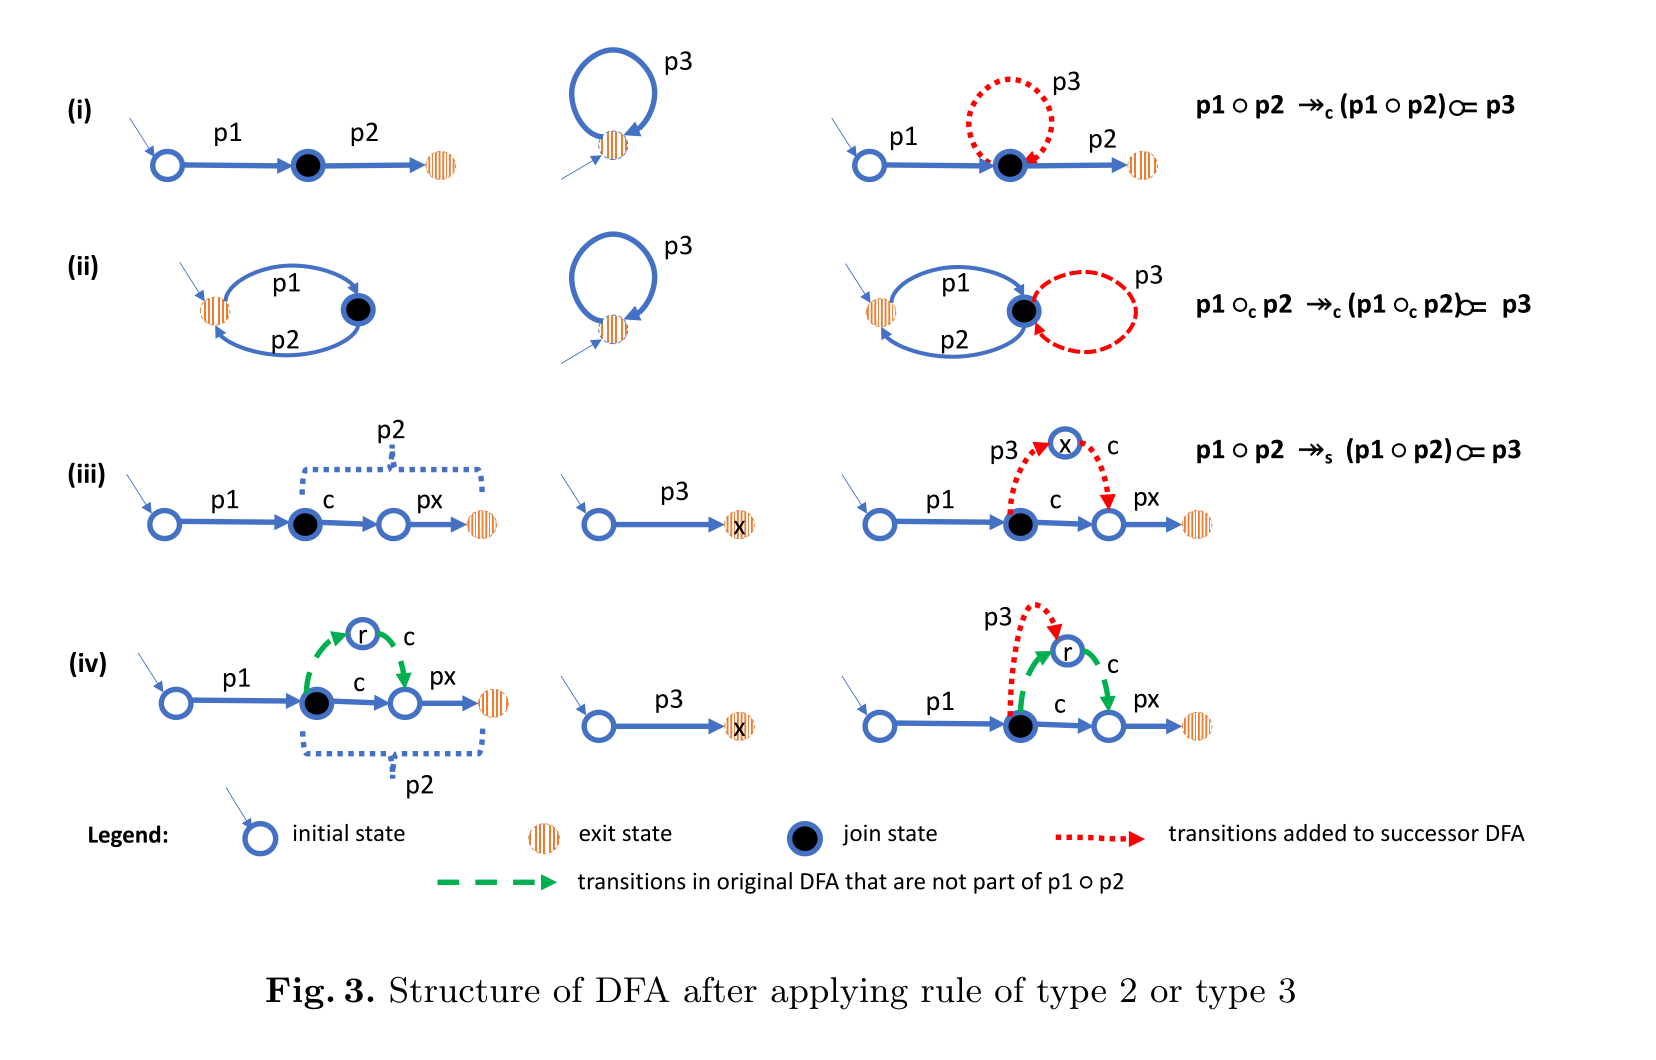
\includegraphics[width=0.6\linewidth]{2.png}
	\end{figure}
\end{frame}

\begin{frame}
	\frametitle{Deviations from the PRS framework}
	\begin{itemize}
		\item Incorrect pattern creation:threshold
		\item Simultaneous rule applications
	\end{itemize}

	\begin{figure}
		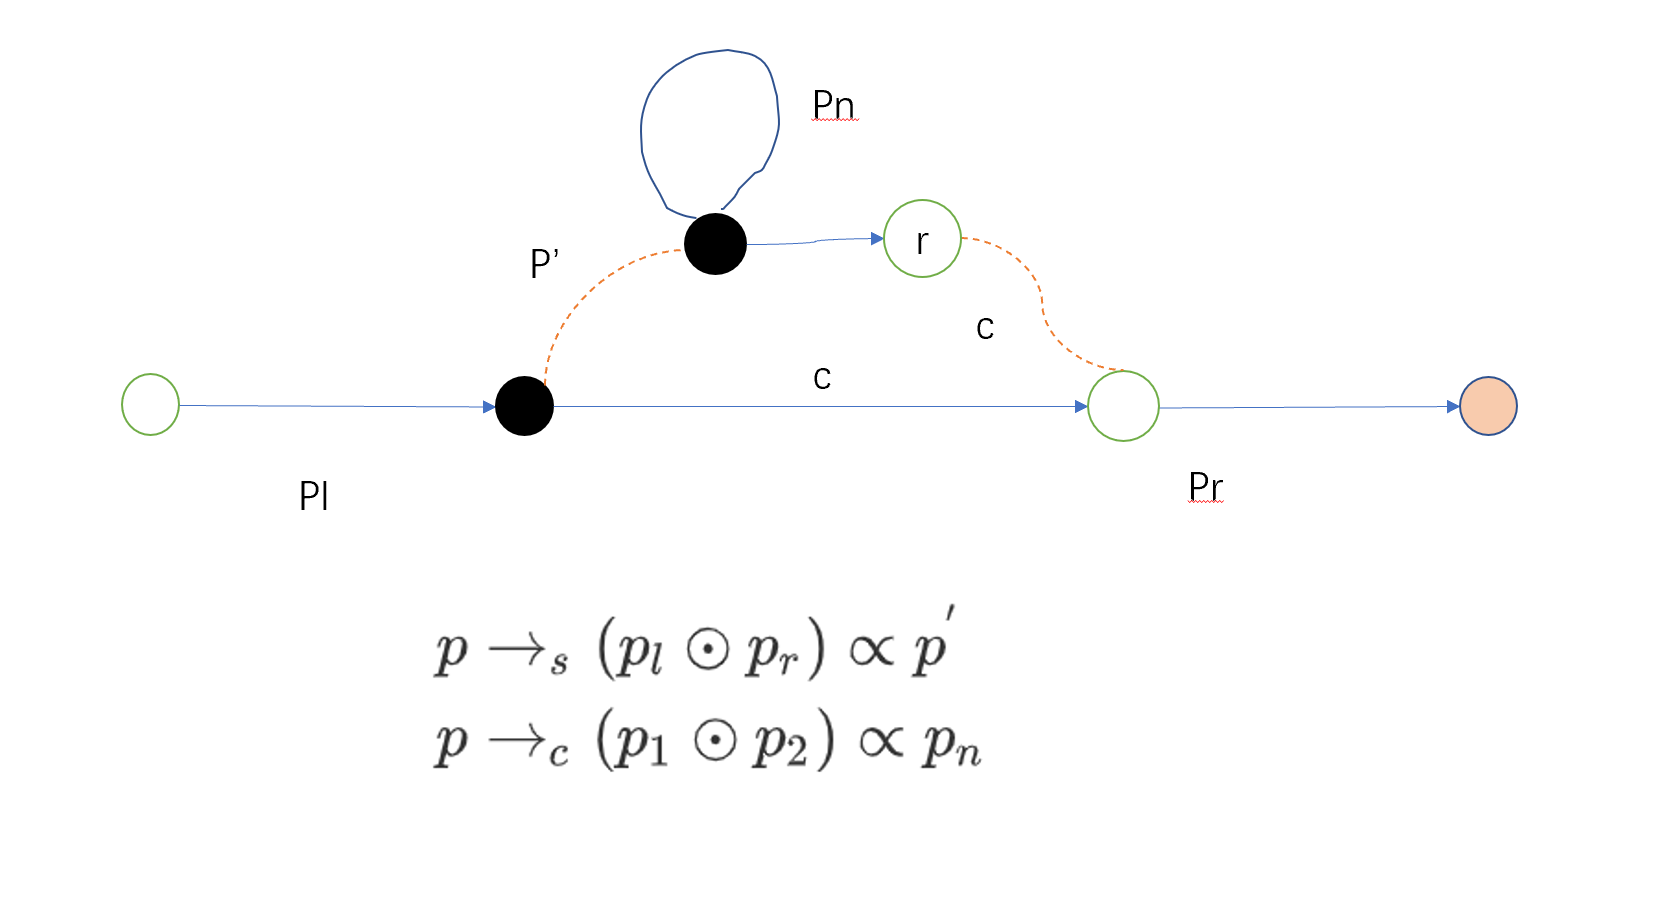
\includegraphics[width=0.6\linewidth]{6.png}
	\end{figure}
\end{frame}

\subsection{Converting a PRS to a CFG}
\begin{frame}
	\frametitle{algorithm}	
		\begin{itemize}
			\item $CFG = <\Sigma,N,S,Prod>:N,Prod?$
			\item $\forall p \in P, G_p = <\Sigma_p,N_p,Z_p,Prod_p>$
			\item $P_Y \subseteq P$:LHS of some rule of type(2).
			\item $N = \{S,C_S,E_S\} \bigcup\limits_{p \in P}\{N_p,E_p\}\bigcup\limits_{p \in P_Y}\{C_p\}$
			\item $S ::= E_S, S ::= C_SE_S,C_S::= C_SC_S$
			\item For $\perp \rightarrow p^{I}, E_S:: = Z_{p^I}$. If circular,$\perp \rightarrow p^{I}, C_S:: = Z_{p^I}$
			\item For each $p \rightarrow_{c}\left(p^{1} \odot p^{2}\right) \propto p^{3},p \rightarrow_{s}\left(p^{1} \circ p^{2}\right) \propto p^{3}$,$Z_p:: = Z_{p_1}E_pZ_{p_2},E_p:: = Z_{p_3}$
			\item For $p \rightarrow_{c}\left(p^{1} \odot p^{2}\right) \propto p^{3}$,creates $Z_p:: = Z_{p_1}C_pE_pZ_{p_2}, C_p::= C_pC_p, C_p:: = Z_{p_3}$
			\item $Prod =\{\bigcup\limits_{p \in P}\} \cup Prod'$  
		\end{itemize}	
\end{frame}

\section{Result}
\begin{frame}
	\begin{itemize}
		\item Every RE-Dyck language can be expressed by a PRS.
		\item But not every CFL can be expressed by a PRS,such as $H = \{a^ixb^i,i \in \mathbb{N}\}$.
		\item The construction above does not necessarily yield a minimal CFG $G$ equivalent to $P$.
	\end{itemize}

	Experiment setting:
	\begin{itemize}
		\item vote:2
		\item Sample: weight version of CFG, N=10000
		\item 2-layer LSTM,hidden dimension = 10, input dimension = 4
	\end{itemize}
\end{frame}

\begin{frame}
	\begin{columns}
		\begin{column}{.5\textwidth}
			\begin{figure}
				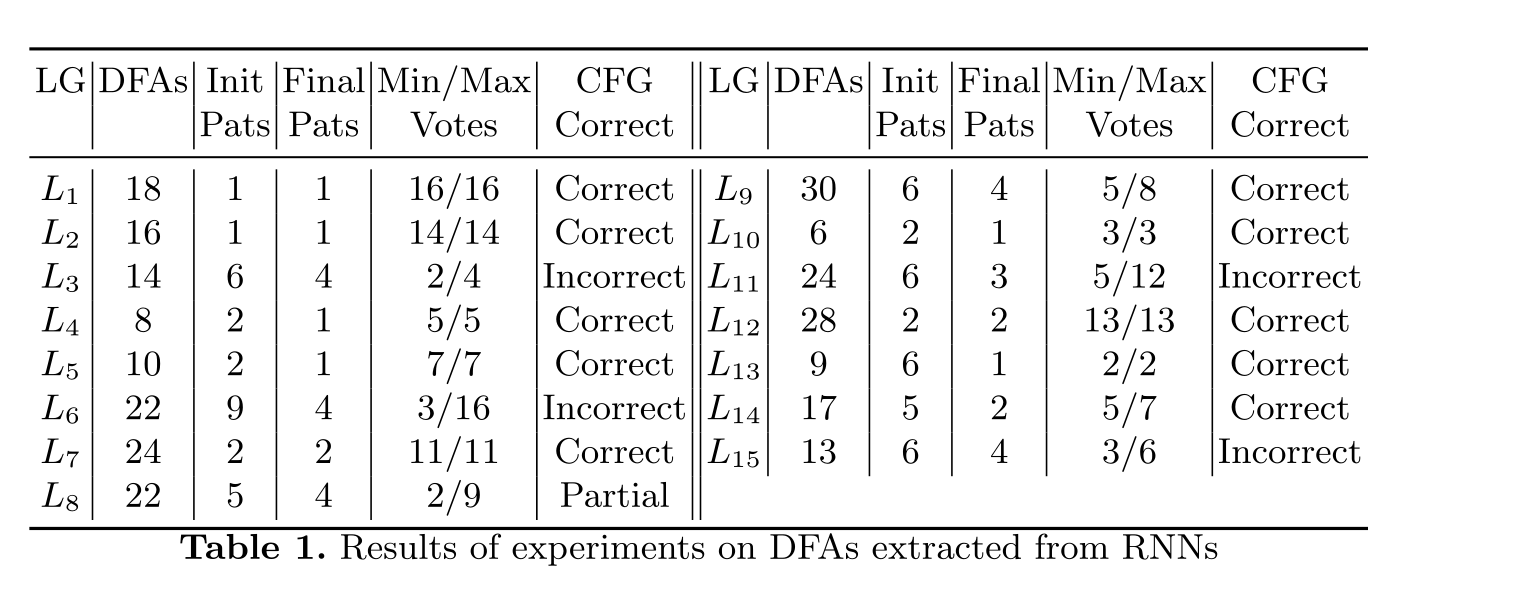
\includegraphics[width=1\linewidth]{7.png}
			\end{figure}
		\end{column}
		\begin{column}{.5\textwidth}
			language of $X_nY_n$:
			\begin{itemize}
				\item $L_1-L_3:(a,b),(a|b,c|d),(ab|cd,ef|gh)$
				\item $L_3-L_6:(ab,cd),(abc,def),(ab|c,de|f)$
			\end{itemize}

			Dyck and RE-Dyck language:
			\begin{itemize}
				\item $L_7-L_9:$Dyck languages (excluding $\epsilon$) of order 2 through 4
				\item $L_{10}-L_{11}:$ RE-Dyck of order 1,$L_{10},R_{10} = (abcde,vwxyz),L_{11},R_{11} = (ab|c,de|f)$
			\end{itemize}
		\end{column}
	\end{columns}
\end{frame}

\begin{frame}
	Variations of the Dyck languages:
		\begin{itemize}
			\item $L_{12}:$ alternating single-nested delimiters,([([])]) or [([])]
			\item $L_{13}-L_{14}:$Dyck-1,2 with additional neutral tokens a,b,c that may appear multiple Times
			\item $L_{15}:$Dyck-1,additional neutral tokens abc or d;(abc()())d,a(bc()())d
		\end{itemize}
\end{frame}

\begin{frame}
	\begin{itemize}
		\item Alternating Patterns:$L^*$ extraction had ‘split’ the alternating expressions
		\item Simultaneous Applications:very large counterexample was returned to $L^*$:
		\item Missing Rules: large number of possible delimiter combinations($L_8$)
		\item RNN Noise:d be included between every pair of delimiters in DFAs($L_{15}$).
	\end{itemize}
\end{frame}

%------------------------------------------------
\begin{frame}
\hfill
\center{\Huge{\calligra{\Huge{Thank you}}}}
\linespread{3}\selectfont
\end{frame}
%----------------------------------------------------------------------------------------
\end{document}